% The Thesis Introduction
% Lit review, rationale, permission from copyright holder for figs if unchanged, all should be modified, should close with statement of aims to be addressed
\graphicspath{{chapters/1.Introduction/figures/}}

\begin{savequote}[75mm]
Hofstadter's Law: It always takes longer than you expect, even when you take into account Hofstadter's law
\qauthor{- Douglas Hofstadter: \textit{G\"odel, Escher, Bach: An Eternal Golden Braid, 1979}}
\end{savequote}

\chapter{Introduction}

%Diversity of endosymbiosis - its a lot of things, complex, ununified, lots of research
% most prevalent examples shape the eukaroytes - plastids and mitochondria
% hard to study as things have been fixed
%Paramecium biology
%Chlorella biology
%Knowledge of their interaction
%http://www.nature.com/nature/journal/vaop/ncurrent/full/nature15205.html

\section{Endosymbiosis}

%http://judgestarling.tumblr.com/post/79135526488/the-phylogeny-of-everything-the-origin-of - some good material and refs on euk origin



\subsection{What is endosymbiosis?}

Endosymbiosis has proven one of the most fundamental processes in the evolution of the
eukaryotic cell \citep{Timmis2004,Lane2007a,Martin1998b,Archibald2015}. It has both shaped the global climate and
created the cellular context in which specialised multicellular organisms have evolved.

Endosymbiosis is a special case of symbiosis, which results in a long-term stable interdependent 
living together (``sym/σύν'' -- together, ``bios/βίωσις'' -- living) of two or more 
organisms to a point of mutual benefit \citep{DeBary1869,Pound1893} (although many now expand 
this definition beyond mutualism to include other categories of biological interactions \citep{Leung2008,OMalley2015}).
What differentiates endosymbiosis from symbiosis in general is that one partner (the endosymbiont) lives wholly
inside (``endo/ἔνδον'' - inside) of another (the host). This ``inside'' can refer to symbionts either living intracellularly
or within the tissues of multicellular organisms.  However, it excludes niches such as the digestive tract of metazoa as 
as this can be considered as an external surface of the host. These latter symbionts are occasionally termed ectosymbionts.
\begin{table}[h]
    \begin{tabular}{|c|c|}
        \hline
        \textbf{Interaction Name} & \textbf{Interaction Outcome} \\ 
        \hline
        Mutualism               & \((+, +)\)  \\
        Antagonism              & \((+, -)\)  \\
        Competition             & \((-, -)\)  \\
        Commensalism            & \((+, 0)\)  \\
        Amensalism              & \((-, 0)\)  \\
        Neutralism              & \((0, 0)\)  \\ 
        \hline
    \end{tabular}
    \caption{An overview of the categories of biological interaction and the effect they have on the two interacting
        biological units, which may be anything from individual species to whole populations. The outcome column 
        contains a tuple relating the effect an interaction has on a pair of interacting biological units. 
        This ``effect'' is often assessed in terms of metrics such as individual fitness, population size and/or
        growth rate.
        Note: parasitism and predation are mechanisms by which an antagonistic interaction may take place \citep{Abrams1987}
        in the same sense that endosymbiosis is a mechanism by which a mutualistic interaction can take place.
        In reality most interactions will not fall neatly into one of these categories and throughout it's duration
        will often display characteristics of multiple categories \citep{Leung2008}}. 
   \label{tab:biointeractions}
\end{table}

There is a considerable variety of endosymbiotic relationships in nature. These relationships can encompass many different
degrees of host-symbiont integration, interdependence and ecological interaction types (see \cref{tab:biointeractions}.  
Even if we restrict ourselves to endosymbioses that are largely ``mutualistic'' (noting that the exact nature of
a certain endosymbiosis is highly dependent on the exact ecological context at a particular point of time and doesn't
always neatly quantize \citep{Leung2008})\footnote{Even as early as this we 
    it is worth briefly addressing a common motif of modern biology: discrete schemas applied to 
    continuous distributions.  These biological quantizations are prone to error (fuzzy delineations)
    and are constantly challenged by novel discoveries which exhibit a mosaic of category features.  
    There are a plethora of examples of this including classification of 
    mitochondria-related organelles \citep{Maguire2014}, types of biological interactions 
    (see \cref{tab:biointeractions}), and the numerous species concepts \citep{DeQueiroz2007,Boenigk2012}.
    That is not to say biological quantization is without utility or is a futile task.  Indeed, as long as there is a clarity to 
    the application and synthesis of these schema then they form a critical (epistemological) framework upon which further 
    research and communication can build. 
    However, care must be taken not to forget that these schema do not reflect reality and can inadvertently obscure
    the grey areas \citep{Leung2008}.  Generally, we must ensure that the schema used are in concordance with the practicalities of the 
discussion at hand (generalising on \citep{Boenigk2012}).}) there is broad range of characteristics.
For example, in terms of interdependence of host and endosymbiont you could construct a spectrum with ``incidental'' endosymbioses 
such as bacterial escape of digestion in macrophages at one extreme and at the other obligate systems such as the mitochondria or chloroplast 
where host and symbiont are essentially a unified unit of selection.  In the middle of such a spectrum you could find facultative endosymbioses
where each partner is capable of, and does, live aposymbiotically for extended life phases e.g. Rhizobia bacteria and legume (Fabaceaea) plants 
(reduction of atmospheric \(N_{2}\) to ammonia \citep{Hirsch1992} in exchange for host-derived carbon sources such as malate and succinate) \citep{Prell2006})

Likewise, an endosymbiosis may be highly metabolically, genomically, and life history integrated but only moderately interdependent (such as facultative Rhizobia nitrogen fixation which takes place
in carefully controlled specialised root nodule structures \citep{Crespi2008}.  However, generally interdependence and integration correlate reasonably
well due to the increased selective pressure to minimise lethal aberrant interactions that comes with interdependence.  This can be seen 
in the extreme of host-symbiont integration: that of the endosymbiotic organelles, which are so highly integrated they were considered part of the cell by
mainstream scientific establishment until only relatively recently.

% This is principally in terms of
%metabolic connectivity (direct connections between biosynthetic and other metabolic pathways betwee partners) \citep{Karkar2015},
%lifecycle integration, and genomic integration (transfer and/or incorporation of genetic material 
%between partners) \citep{Timmis2004} (although all categories overlap).

\begin{figure}[h!]
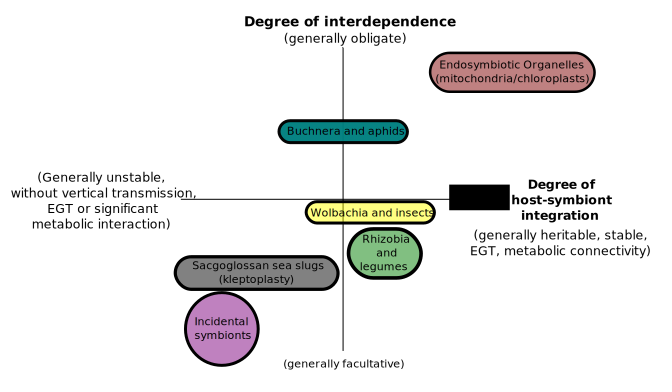
\includegraphics[width=\textwidth]{integration_vs_dependence.pdf}
    \caption{ 
        %%Sacoglossan sea slugs aren't really secondard endosymbionts as they only keep plastid of algea \citep{Christa2014}
        %%NEEDS WORK AS A FIGURE AND CITATIONS FOR CAPTION
        %% See figure in stoecker2009 about the spectrum of acquired phototrophy in proitsts
        Plot demonstrating a fragment of the diversity of endosymbioses and specifically hi-lighting the possibility of
        a well integrated by facultative endosymbiosis.
        Host-symbiont integration is a rough measure of how connected the host and symbiont have become genomically, metabolomically
        and in terms of life history.  Whereas, interdependence is a approximate measure of the degree to 
        which the relationship is necessary for life of organisms involved. 
        It should be noted that both axes can be highly reliant on specific ecological and environmental context.
    }
    \label{fig:integrationvsdependence}
\end{figure}

Intracellular endosymbionts can be found inhabiting multiple host-compartments from nakedly in the cytoplasm, to host-derived
vacuolar compartments (often from secretory and endocytic systems) (e.g. \citep{Kodama2009a}) along with a range of 
host oraganelles including the endoplasmic reticulum \citep{Vogt1992}, Golgi body \citep{Cho2011},
mitochondria \cite{Sassera2006}, chloroplast \citep{Wilcox1986} as well as the nucleus 
(first discovered in \textit{Paramecium} \citep{Schulz2015}).
Owing to the endosymbiotic origin of the chloroplast and mitochondria it becomes apparent
that there can be multiple ``layers'' of endosymbiosis. A primary endosymbiont is an endosymbiont that is the direct
endosymbiont of the host (e.g. the mitochondria to eukaryotes) whereas a secondary endosymbiont is the endosymbiont of
an endosymbiont.
The layers of endosymbioses can get impressively deep, for example, bacterial endosymbionts have been identified within the 
chloroplast stroma (cyanobacterial endosymbiont) of dinoflagellates (e.g. \textit{Woloszynskia pascheri} \citep{Wilcox1986})
In turn, dinoflagellate plastids have been discovered that are likely the product of tertiary endosymbioses \citep{Gabrielsen2011} 
with higher-order events hypothesised in related groups \citep{Stiller2014}.
Therefore, bacteria like this could be the endosymbiont of an endosymbiont of an endosymbiont of an endosymbiont (quaternary) or
higher.

With this considerable diversity it is perhaps not surprising that endosymbioses have been discovered featuring partners from all 3 domains of cellular life. %side-steppin the ole viruses thing 
However, with the exception of one extant Bacteria-Bacteria endosymbiosis \citep{vonDohlen2001}, typically the majority of known
endosymbioses feature a eukaryotic host\footnote{There are however many examples of mutualistic symbioses which are Bacteria-Bacteria (e.g. biofilms \citep{Watnick2000}),
    Bacteria-Archaea (e.g. anaerobic methanotrophic archaea and sulphate-reducing bacteria likely responsible
    for a large proportion of global methane consumption \citep{Boetius2000,Knittel2009} and SM1 
    euryarchaea/\textit{Thiothrix} sp. sulphide-oxidising bacteria \citep{Henneberger2006,Wrede2012}), 
    and at least one example of Archaea-Archaea (\textit{Igniococcus hospitalis/Nanoarchaeum equitans} \citep{Huber2002}. 
    Interestingly \textit{Igniococcus} is the first identified case of an energised outer-membrane in 
    double-membrane bound archaea or bacteria, a significant finding for the development of theories of
eukaryogenesis \citep{Kuper2010})} but can include endosymbionts from all 3 domains.
For example:\footnote{Although with all these example, it is important not 
    to consider an endosymbiotic relationship 
    in isolation from other endosymbionts present in the same host.
    There are examples where facultative ``secondary endosymbionts'' 
    are able to compensate for the loss of an obligate endosymbiont \citep{Koga2003}.  Symbiont-symbiont 
    interactions have been found to play a role in determining which endosymbionts are capable of establishing themselves 
    in a certain host and can even be capable of generating additional phenotypes e.g. the R-bodies of ``killer'' \textit{Paramecium} 
    species which may be a product of an interaction between the \textit{Paramecium} host, \textit{Caedibacter} and a bacteriophage
    \citep{Schrallhammer2009}. %Hydra system is another example}
}
\begin{itemize}
    \item Eukaryote-Archaea \citep{Moissl-Eichinger2011}
    \begin{itemize}
        \item Methanogenic archaea within various ciliates species (e.g. \textit{Plagioplya frontata}) \citep{Fenchel1992,Lange2005}
        \item \textit{Cenarchaeaum symbiosum} within the tissues of marine sponges \citep{Preston1996,Wrede2012}
    \end{itemize}
        \item Eukaryote-Bacteria 
    \begin{itemize}
         \item \textit{Hartmannella} and it's intranuclear endosymbiont \textit{Candidatus Nucleicultrix amoebiphilia} \citep{Schulz2014}
         \item the most famous pairing of mitochondria and plastids
    \end{itemize}
    \item Eukaryote-Eukaryote
    \begin{itemize}
        \item The fungi \textit{Diplodia mutila} which aids herbivory resistance in the palm \textit{Iriartea deltoidea} in lowlight
            conditions but becomes pathogenic if host is well lit \citep{Alvarez-Loayza2011}
        \item Red alga derived plastids in brown algae \citep{Dorrell2011}
        \item Numerous examples of algal mediated acquired phototrophy in ciliates \citep{Johnson2011}
    \end{itemize}
\end{itemize}

Endosymbiosis is the one of the most significant evolutionary processes in eukaryotic cell.
It offers a means for eukaryotes to benefit from the extensive metabolic diversity
present in the bacterial and archael pangenome, especially the only known forms of primary energy
production - photosynthesis and chemosynthesis \citep{Wernegreen2012}.

\subsection{Plastid Endosymbioses}
Most molecular evidence currently points towards a single primary endosymbiotic event between a phagotrophic ancestral
eukaryote (with mitochondria and developed endomembrane system \citep{Rockwell2014}) and a cyanobacteria (blue-green algae) as giving rise to 
the archaeplastida (that is the green algae, red algae, glaucophytes and land plants \citep{Green2011}) and their double membrane bound plastids \citep{Keeling2013}.   
While, this event is one of the must fundamental events in the evolution of life in and of itself it is only capable of explaining a small 
proportion of the diversity of plastids across the eTOL \citep{Keeling2013}
Apart from one other putative primary endosymbiosis in \textit{Paulinella chromatophora} (a euglyphid amoeba with photosynthetic 
chromatophores that are vertically inherited, synchronised to host and bear a much stronger molecular and morphological resemblance to reduced 
cyanobacteria than the chloroplast of the archaeplastida \citep{Kies1979,McFadden2014}) all other oxygenic phototrophs 
(as well as several non-photosynthetic but plastid bearing pathogens \citep{Sato2011}) have arisen by secondary or 
higher order endosymbioses \citep{Hoshina2009}.
Secondary endosymbioses are those in which another eukaryotic lineage has engulfed a primary plastid bearing algae and reduced and integrated them in a 
simulacrum of primary endosymbiosis, occasionally serially \citep{Keeling2010}. This and subsequent loss of membranes leads to the range of membrane
layer numbers around plastids in various eukaryote lineages \citep{Keeling2013}.  %Often in the endomembrane system
This secondary order plastid endosymbioses have occurred independently in divergent eukaryote lineages e.g. chloroarachniophytes and euglenids, and 
an unresolved number of times in the the set of cryptomonads, haptophytes, stramenopiles, dinoflagellates and apicomplexans \citep{Keeling2013}.  
As well as an uncertain number of higher order endosymbioses in the dinoflagellates \citep{Keeling2013}.

Therefore, understanding the mechanisms and evolution of secondary photosynthetic endosymbioses would provide important insight into the evolution of a considerable number of eukaryotic lineages.  Unfortunately, most extant examples feature endosymbioses within which metabolic co-dependence has already become fixed
masking the potential mechanisms through the endosymbiosis may have originated.  
Facultative systems such as the \textit{Chlorella} endosymbionts of \textit{Paramecium bursaria} offer a potential avenue to investigate secondary 
photosynthetic endosymbioses at an earlier stage before metabolic co-dependence has become fixed (while acknowledging the impossibility of 
interrogating events that have already occurred within the correct ecological context.
Furthermore, as the ancestral protist involved in the primary plastid endosymbiosis likely exhibited a similar life style to serially phagotrophic
\textit{Paramecium} and would initially at least have been mixotrophic (combining phagotrophy with phototrophy via the newly acquired plastid \citep{Rockwell2014} in the same manner as \textit{Paramecium bursaria} (and other mixotrophic ciliates \citep{Johnson2011}) the study of the \textit{Paramecium bursaria}-\textit{Chlorella} system offers potential insight into this early and fundamental stage of eukaryote evolution.

\section{\textit{Paramecium bursaria}}
\textit{Paramecium} are large (\(50-330\mu m\)) phagotrophic single-celled eukaryotes belonging %size from wiki...
to a genetically diverse \citep{Prescott1994} sub-grouping of the alveolates known as the ciliates (see \ref{fig:tol}).
They have been studied since the invention of microscopy \citep{Gortz2009} (first recorded by a contemporary of van Leeuwenhoek 
see \ref{fig:huygens}) and are some of the longest-standing model unicellular eukaryotes.  They have been used
to study everything from mutagenisis and developmental genetics, to genomics rearrangement and epigenetics \citep{McGrath2014}. 
As such have a well-developed methodological \citep{Sonneborn1970} and theoretical literature along with 
several available genomes (see \ref{fig:paramecium_genomes} for genomes and their relative relationship to \textit{P. buraria}). %Why study section

\textit{Paramecium bursaria} ``the green \textit{Paramecium}'' is distinguished from most\footnote{
    There is at least one other species, \textit{Paramecium chlorelligerum}, that harbours a different green algae (\textit{Meyerella}) \citep{Kreutz2012}
    and owing to the multiple origins of algal symbionts in \textit{P. bursaria} \citep{Hoshina2009} and the general prevalence of mixotrophy
    in ciliates \citep{Johnson2011} there are likely others yet to be discovered.
}other \textit{Paramecium} by the distinctive stable, heritable secondary photosynthetic endosymbiosis it maintains with several species of 
the green algae \textit{Chlorella}.  
Each \textit{P. bursaria} \(100-160\mu m\) \citep{Jennings1939} cell contains \(\sim 300\) endosymbiotic algae maintained in individual perialgal vacuoles (PV) around the cell cortex \citep{Hoshina2009}.

\begin{figure}[h!]
    \caption{\textbf{A}: Carving of Christiaan Huygens (1629-1695), the prominent Dutch Golden Age mathematician and scientist and contemporary of Antoni van Leeuwenhoek, from a medallion by Jean-Jacques Cl\'erion 1679 (reproduced from \citep{Huygens}). \textbf{B}: Likely the first sketch of the micro-organism that we now know as \textit{Paramecium} by Christiaan Huygens in a letter (No. 2133, 11th of August 1678) to his father Constantijn Huygens. An approximate translation of the accompanying text goes as follows ``I have twice seen in this water an animal 10 times as large as the others and with feet all over its body and a narrow form. 4 or 5 feet stirred even when the animal was at rest. It moves as fast as the others, turning and spinning in the water. Hartfoecker thinks he may have discovered the same species in `semine corrupto' (as a dried out husk?).'' (reproduced from \citep{Huygens}). \textbf{C}: 8 of the 10 volumes of the collected correspondences of Christian Huygens as prepared for the Dutch Society of Sciences and published from 1888-1905)}
    \label{fig:huygens}
\includegraphics[width=\textwidth]{Christiaan_Huygens_combined_figure.pdf}
\end{figure}

\begin{figure}[h!]
    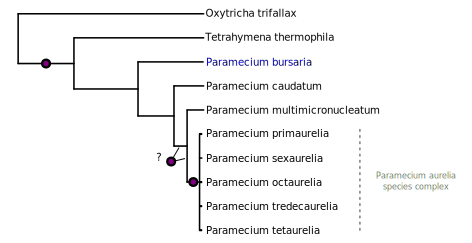
\includegraphics[width=\textwidth]{paramecium_genomes.pdf}
    \caption{Modified phylogeny redrawn from \citep{Fokin2004,Aury2006,McGrath2014}
             Showing the relative relations of ciliate species with genomic/transcriptomic resources and hypothesised WGD event locations with a purple dot.
             Specifically 2 strains of \textit{Paramecium tetaurelia} \citep{Aury2006}, assemblies for 
             \textit{P. caudatum}, \textit{P. multimicronucleatum}, and \textit{P. aurelia} complex species \textit{P. sexaurelia},
             \textit{P. primaurelia}, \textit{P. octaurelia} and \textit{P. tredecaurelia} on ParameciumDB (as of 05/03/2015) \citep{Arnaiz2011}.
         As well as \textit{Tetrahymena thermophila} \citep{Eisen2006} and \textit{Oxytricha trifallax} \citep{Swart2013}.}
    \label{fig:paramecium_genomes}
\end{figure}

Much like other ciliates, \textit{Paramecium} are covered by cilia. 
These are minute hairlike biochemically heterogeneous organelles capable of sensing the environment and by
beating in co-ordinated metachronal waves of power strokes and recovery strokes \citep{Funfak2015} provide cellular locomotion and, 
in the case of phagotrophic ciliates like \textit{Paramecium}, forcing food bacteria towards
the oral groove (cytopharynx) where they can be phagocytosed \citep{Hamel2011,AubussonFleury2015}. %no phagocytotic ciliates?
\textit{Paramecium} is also capable of rapid locomotion via the expulsion of trichocysts.
These are defensive membrane-bound organelles known as trichocysts containing a crystalline spike which can be 
rapidly ejected into the environment on fusion of trichocyst membrane with plasma membrane \citep{Hamel2011}.

Like other ciliates, including \textit{Tetrahymena}, \textit{Paramecium} deviates from the universal genetic code.
Canonical stop codons TAA and TAG have been reassigned to produce glutamine therefore there is only one stop codon (TGA) but 4 glutamine codons \citep{Salim2008}.  

Another defining feature of \textit{Paramecium}, and ciliates in general, is a unique means of germline sequestration from somatic function 
in the form of ``nuclear dimorphism'' \citep{Jahn2002}.
Specifically, they have two types of nuclei, expression optimised highly polyploid somatic macronuclei (MAC)
and largely silent diploid germline micronuclei (MIC) \citep{Prescott1994}. 

During normal vegetative growth the MIC is densely packed with chromatin, is transcriptionally silent and undergoes
mitosis as standard.  Meanwhile, the MAC reproduces by a non-standard pinching process termed ``amitosis''.  This process
appears to lack any mechanism to ensure equal segregation of chromosomes such as spindle fibres \citep{Kiefer2013}.
On the other hand, during sexual reproduction (in which two compatible \textit{P. bursaria} exchange haploid MIC gametes generated by meosis) the MAC 
degrades and must be reconstituted entirely from the newly formed heterozygous MIC \citep{Jahn2002} (see \ref{fig:pb_sex}).
The exact number of MIC and MAC varies widely by species and genus however, \textit{P. bursaria}
contains a single large MIC which consists of 80 to several hundred chromosomes depending on the exact subspecies \citep{Chen1940}.  

\textit{P. bursaria} reaches sexual maturity after 50-100 fissions \citep{Siegel1960} and will conjugate with another \textit{Paramecium bursaria}
cell of compatible mating type and exchange haploid MIC gametes. Most \textit{Paramecium} have a finite number of vegetative divisions and 
will die if they do not sexually reproduce \citep{Kiefer2013}. Unlike all other studied \textit{Paramecium}, 
\textit{P. bursaria} does not only have 2 mating types and appears to have undergone gene duplication at two unlinked mating type loci.  
Different \textit{P. bursaria} isolates display 2, 4 and 8 mating types \citep{Phadke2009} and form 4 or more mutually 
incompatible groups \citep{Jennings1939}. 
Sexually \textit{P. bursaria} appears to have synclonal inheritance - a strictly mendelian inheritance contrary to the more 
complex epigenetic patterns observed in other \textit{Paramecium} species (that led to much of the early work on epigenetics) \citep{Siegel1960,Phadke2009}.
During conjugation there is minimal cytoplasmic exchange (with no exchange of endosymbionts) \citep{Wichterman1946}. %check this %Conjugants don't typically exchange cytoplasm (except under special conditions (such as antibody treatments \citep{Harrison1945}) .%\citep{Siegel1963}
Contrary to other \textit{Paramecium} species, which undergo autogamy after 75 rapid replications \citep{Sung2012} or 30-35 while starving
\citep{Berger1986}, \textit{Paramecium bursaria} has not been found to naturally undergo autogamy \citep{Siegel1963,Yanagi2004} 
but it can be induced by treatment of methyl cellulose \citep{Yanagi2004}

In \textit{Paramecium} the haploid size and complexity of the MIC is greater than that of the MAC as a result elimination 
of approximately 20-30\% of DNA during reconstitution of the MAC from the MIC.  
Eliminated sequences are known as internal eliminated sequences (IES) and are a mixture of 
transposon-related repetitive sequences and nongenic single-copy sequences resulting in a gene dense low-repeat MAC \citep{Kiefer2013}.   
Similarly, the MAC has a greater number of shorter chromosomes than the MIC due to chromosomal fragmentation during DNA elimination by imprecise
deletion of internal DNA segments followed by rejoining or telomere addition \citep{Kiefer2013}.
This process involves 3 steps is observed in \textit{P. tetaurelia} and features
a special class of small RNAs (scnRNAs) \citep{Kiefer2013}:
\begin{itemize}
    \item DNA amplification to high ploidy.
    \item DNA elimination pathway 1: accurate removal of short unique-copy elements (IES, internal eliminated sequences) that run through coding and non-coding sequences. This is achieved using bounding 5'-TA-3' dinucelotides to target double-stranded breaks and subsequent end-joining \citep{Mayer1999,Betermier2004}
    \item DNA elimination pathway 2: imprecise removal of large DNA regions (often containing transposable elements) in a manner similar
        to transposon silencing in other eukaryotes.  This process likely involves short ncRNAs targeting heterochromatin formation via histone methylation to induce fragmentation.  This fragmentation is subsequently repaired via the addition of new telomeres \citep{Duret2008}.
\end{itemize}
This process involves a special class of meiosis specific small RNAs (scnRNAs) which target aspects of DNA elimination \citep{Kiefer2013}.


While the MIC appears to vary in size between subspecies of \textit{P. bursaria} the MAC is roughly the same
size and generally contains 10-30 times the amount of DNA than the diploid MIC \citep{Cullis1972}.  
Therefore, the MAC of \textit{P. bursaria} is likely 20-60n (in contrast to the 800n MAC ploidy found in \textit{P. tetaurelia} \citep{Duret2008}).
The MAC genome is likely to be somewhere between 20 and 100Mb and contain somewhere between 
18,000 and 40,000 genes based on the size of the \textit{Tetrahymena} \citep{Eisen2006}, 
\textit{P. tetaurelia} \citep{Aury2006}, \textit{P. caudatum} \citep{McGrath2014} and \textit{Oxytricha} \citep{Swart2013} MAC genomes.

We can infer other likely features of the \textit{P. bursaria} MAC genome from the \textit{P. tetaurelia} sequencing project.
Specifically, it is likely AT-rich (28\% GC in \textit{P. tetaurelia}), compact (78\% coding density in \textit{P. tetaurelia}),
mostly repeat free with small intergenic regions and many short introns (e.g. 25bp IES elements) \citep{Aury2006}.  
There is also likely to be evidence of at least 1 whole genome duplications (WGD) (an ancient WGD before the divergence of 
\textit{Tetrahymena} and \textit{Paramecium} clades but not the 2 most recent WGD (see \cref{fig:paramecium_genomes}) 
giving rise to the \textit{P. aurelia} complex) with a moderate 
level of conservation to gene synteny and duplicated gene retention 
(weakly correlating with a genes GC\%, expression level and functional class) \citep{Aury2006,McGrath2014}.
%No clear evidence of algal ancestry - throwing doubt on the ``chromalevolate'' hypothesis or suggesting total loss
%of these features 
\textit{P. bursaria} is also likely to be have a high level of replication fidelity and relatively low rate of base-substitution mutation,
traits found in \textit{P. tetaurelia}, as \textit{P. bursaria} shares ciliate specific modifications to the active sites
of B-family polymerases \(\alpha, \zeta\), and the proofreading exonuclease of DNA polymerase \(\epsilon\) believed to be adaptions to
improve replication fidelity and a necessary adaptation when maintaining a separate germline \citep{Sung2012}.

\begin{figure}[h!]
    \caption{
        Figure redrawn and modified from \citep{Duret2008}.
        During normal vegetative growth \textit{Paramecium bursaria} (and other \textit{Paramecia}) divide by binary fission with the MAC
        elongating and ``pinching'' off in a process distinct from mitosis (known as amitosis) while the MIC undergoes mitosis.
        As the cell pinches before cytokinesis an unknown septum forms at the ``neck'', this stops cytoplasmic streaming which induces
        the endosymbionts to begin to divide. Cytokinesis then occurs largely simultaneously in host and endosymbionts \citep{Kadono2004,Takahashi2007}.
        The sexual cycle involves conjugation of compatible mating types (taking around an hour and lasts 24-48 hours \citep{Jennings1939}) 
        which triggers two-rounds of meosis of the MIC with
        one product disintegrating after each division so only a single haploid MIC remains. This undergoes mitosis to produce male and
        female gametes. Male gametes are then reciprocally exchanged between mating cells and fuse with the respective female gamete to 
        create a syncaryon. Each syncaryon divides onces and one product disintegrates before undergoing two subsequent divisions.
        Two products differentiate into MACs by programmatic reorganisation, conjugants split and a normal binary fission occurs 
    restoring normal 1 MAC and 1 MIC \citep{Siegel1963} }%based on }
    \includegraphics[width=\textwidth]{paramecium_bursaria_sexual.pdf}
    \label{fig:pb_sex} 
\end{figure}

There is no established methodology in \textit{Paramecium} to transform the MIC genome so the only available reverse genetic methodology is that of
gene knock-down with RNA interference (RNAi) \citep{Marker2014a}.  
However, RNAi can be induced by one of two distinct but overlapping RNAi systems in \textit{P. tetaurelia} \citep{Marker2014a}.
This is by microinjection\footnote{ This common RNAi pathway can be invoked by both Direct injection of dsRNA into the cytoplasm only triggers transient silencing, likely due to growth related dilution \citep{Galvani2002}.
Heritable silencing cannot be triggered by dsRNA (possibly due to insufficient RDR activity and absence of H3K9 histone factors in MIC) in \textit{Paramecium tetaurelia} \citep{Kiefer2013}).}
of homologous transgenes (transgene-induced silencing) or by feeding \textit{Paramecium} cells
\textit{Escherichia coli} transformed to produce sense and antisense transcripts for the target gene respectively \citep{Galvani2002}
Furthermore, natural exogenous ssRNA in food bacteria of \textit{P. tetaurelia} has been observed to produce low levels of silencing, therefore this mechanism
is a likely a form of natural gene regulation used by \textit{Paramecium} \citep{Carradec2015}.
As \textit{P. bursaria} shares the initial ancient WGD with \textit{P. tetaurelia} \citep{Aury2006} based on \textit{P. tetaurelia} genes that are the 
product of this WGD it currently or previously will have possessed: a pair of Dicer/Dicer-like proteins, 6 pairs of Piwi genes and a single RdRP \citep{Marker2014a}.
Therefore, RNAi is likely available in \textit{P. bursaria} as a means of testing predictions generated through transcriptomic and genomic investigation.

%$Endogenous silencing pathway in \textit{Paramecium} requires an RNA-dependent RNA polymerase (encoded by RDR3 \textit{Paramecium}) for
%$accumulated of endogenous siRNAs.  siRNAs homologous to gene junction regions have been observed in \textit{Paramecium}. 
%$dsRNA is the most likely trigger for transgene-induced silencing observed in \textit{Paramecium}
%However, Forward genetic screen experiments conducted by Marker \textit{et. al.} \citep{Marker2014a} identified the presence of two distinct
%but overlapping RNAi mechanisms within \textit{Paramecium tetaurelia} triggered by high-copy transgenes and feeding by dsRNA producing bacteria respectively.
%Interestingly, they identified all dsRNA mediated RNAi specific factors as non-essential but transgene induced silencing involved factors appeared 
%to be essential \citep{Marker2014a}.

%Naturally dsRNAs can occur by RNA-based RNA polymerisation (typically viral in origin), hybridisation of complementary RNAs such as 
%overlapping transcripts that can arise from transcription of repetitive sequences like transposons or transgene arrays, and by self-complementary hairpin 
%forming repeats \citep{Meister2004}.
%These dsRNAs are transformed into short 21-28nt RNA fragments via Dicer mediated endonucleolytic cleavage known as siRNA, rasiRNA and miRNAs respectively \citep{Meister2004}.
%Many genes that produce miRNAs are evolutionarily conserved leading important gene regulation.
%
%Additionally, many organisms, including \textit{Paramecium tetaurelia} have been discovered to undergo RNAi in response to exogenous dsRNAs \citep{Galvani2002}.
%In order to amplify the silencing response these primary siRNAs are frequently replicated in the host organisms via RNA-dependent RNA polymerases (Rdr). \citep{}
%
%An important regulator of transcript processing is that of small RNAs. Typically long dsRNA molecules are processed by
%Dicer-mediated endonucleolytic cleavage into 21-28nt short-interfering RNAs (siRNAs) 
%
%Via Argonaute effector complexes these siRNAs will target homologous cellular RNAs (of various types) and can subsequently
%play a key role in various forms of gene expression regulation known as RNAi. 
%RNAi consists of both the canonical post-transcriptional gene silencing by targeting homologous mRNAs for degradation or by blocking
%translation by interfering with mRNAs or small ncRNAs as well as transcriptional silencing induced by RNAi of chromatin epigenetic
%modification.
%
%\citep{Carradec2015}
%from direct post-transcriptional silencing, 
%
%will subsequently
%control gene expression 
%
%control gene expression of various

%Rdr2 in specific is necssary for all known siRNA systems as well as sexual reproduction in \textit{P. tetaurelia} \citep{Marker2014a}.

%\textit{P. tetaurelia} encodes a large number different core RNAi factors with 8 Dicer or Dicer-like genes, 17 Piwi genes and 4 RdrP genes \citep{Marker2014a}.
%At least one genomically directed forward genetic study has been completed in \textit{P. tetaurelia} \citep{Marker2014a}.

%$THIS SECTION MIGHT BELONG IN CHAPTER - LEAVE FOR NOW
%$
%$Accumulation of 23nt siRNAs are likely the primary mechanism by which the RNAi system of \textit{Paramecium} induces post-transcriptional silencing of endogenous genes.

%\textit{P. tetaurelia} RNAi machinery processes both single-stranded and double-stranded RNAs from bacterial food it has phagocytosed.
%This suggests exogenously induced RNAi is a natural process in \textit{P. tetaurelia} and potentially other \textit{Paramecium} species.
%primary siRNAs of both strands  processed by Dicer (Dcr1), RNA-dependent RNA polyermases Rdr1, Rdr2 + other factors 
%Dcr1 
%



%\subsection{Endosymbionts in \textit{Paramecium}}
\textit{Paramecium} appears to be particularly competent for endosymbioses with an array of over 60 
genetically diverse putative endosymbionts described \citep{Gortz2009}. 
This is no surprise as ciliates have been known to have bacterial \citep{Gortz2009}, archael \citep{Wrede2012} and 
eukaryotic \citep{Kodama2009a} endosymbionts.
These endosymbionts range in degree from mutualist to parasitic and are cytoplastmic, endomicronucleic,
endomacronucleic and/or perinuclear. 
As a serial phagotroph, \textit{Paramecium} species are liable to infiltration by bacterial capable of escaping or resisting
the phagosomal digestive process. %FOK ALLEN 1988 LYOSOEOME SYSTEM IN PARAMECIUM PRINGER BERLIN 301-324
The \textit{Paramecium bursaria} micronuclei frequently contains bacterial endosymbionts. The closed nature of reproduction
has been suggested as a reason why endonucleobioses are common in paramecium \citep{Gortz2009}
Some endosymbionts exhibit high levels of adaptation, no longer able to be found free-living and with evidence of the genome reduction
distinctive of endosymbiosis \citep{Gortz2009} %No specific citation in revirw
The most frequently identified bacterial endosymbionts in German environmental samples are that of \textit{Holospora  caryophila},
\textit{Holospora obtusa} and \textit{Caedibacter caryophilus}
Several of these endosymbionts have been shown to require specific \textit{Paramecium} genes for maintenance \cite{Fujishima1985}.


%The most famous of these is that of the so-called ``killer endosymbionts'' 
%
%There is no evidence of a plastid or plastid-derived compartment within the ciliates.
%There is some evidence of approximately 16 genes of algal origin within the ciliates 
%Potentially, these could be the remnants of a lost plastid, in the same way remnants of mitochondrial function 
%exist in organisms with highly derived MROs such as \textit{E. histolytica} fitting with the secnario of
%secondary loss of a plastid which could be proved by finding an ancestral photosynthetic lineage.
%In the same way that plastid bearing \textit{Chromera velia} is touted as evidence for the photosynthetic activity
%of an cestral apicomplexans. \citep{Reyes-Prieto2008}

%As mentioned earlier, when one considers the influence Tracey Sonneborn's discovery of non-mendelian
%inheritance non-mendelian inheritance in the related \textit{Paramecium (aurelia)}, where he showed
%cytoplasmic inheritance of features such as cilia orientation\footnote{``Pieces of cortex of Paramecium can be grafted onto a whole cell and
%become integrated, yielding a modified cortical pattern which is maintained through both sexual and asexual reproduction.'' \citep{Beisson1965}}
%
%the development of Margulis' formulation of endosymbiosis \citep{Margulis1998} it is
%quite appropriate that we are revisiting this organism




%Furthermore, Mereschowsky considered a very similar system to \textit{Paramecium bursaria} and 
%its green algal endosymbionts as a key line of evidence in the development
%of his theory of symbiogenisis (the organism \textit{Amoeba viridis}, now known as
%\textit{Mayorella viridis} \citep{
%\citep{Mereschkowsky1905,Martin1999a}
%Indeed protists containing green algae such as \textit{Paramecium bursaria} referenced
%as ``animals on the way to becoming plants.'' were considered by Мережко́вский 
%as ``\textit{ad oculum} examples of the (endo)symbiotic nature of plants \citep{Mereschkowsky1920,Sapp2002}. 




%\section{\textit{Paramecium bursaria} Chlorella Virus}
%
%\textit{Paramecium bursaria} Chlorella Virus (PBCV) is a large icosahedral double-stranded DNA virus belonging to 
%the \textit{Phycodnaviridae}.  It has a 330-kb genome and infects \textit{Chlorella} 
%(specifically PBCV-1 infects \textit{Chlorella} NC64A) inducing host lysis 6-8 hours post infection.
%This leads to the release of approximately 1,000 viral particles of which 25\% are infectious. 
%It lacks a RNA polymerase. \citep{Yanai-Balser2010}
%
%NCLDVs 
%
%Some have cited it as the 3rd member of the PbMr system, acting a strong impetus in the form of a negative
%selection pressure as Chlorella seems to be protected from PBCV when it is an endosymbiont.
%
%
%A close relative (\textit{Acanthocystis turfacea} Chlorella virus 1 ATCV-1) is potentially capable of 
%infecting mammals (including) and potentially impair cognitive function
%If this is true, this would make chloroviruses one of the few known examples of viral groups capable of infecting 
%multiple kingdoms (along with some plant - invertebrate viruses) \citep{Yolken2014}
%
%
%Some evidence of a similar system with other endosymbiont - specifically the Caedibacter0oaranecuyn =0bacvterioahe
%forming the R-body
%R-body formation tripartite raises host fitness eliminated competition Caedibacter phylogeny poor Toxin unknown
%R-body uncoils are kills  \citep{Schrallhammer2009}
%



\section{\textit{Micractinium reisseri} and \textit{Chlorella}}

Chlorella was a key a model organism, forming the basis of the identification 
of the Calvin Cycle \citep{benson1948path}


Green algae have been found displaying all forms of endosymbioses:
transient non-heritable associations \citep{Reisser1993}, 
predation to autotrophy phases during life cycle \citep{Okamoto2005},
kleptoplasts \citep{Schnepf1993}, permanent heritable
association \citep{Siegel1965} and metabolic co-dependence/genetic
amalgamation \citep{Margulis1993}.
Above from \citep{Sano2008}





Sponge and hydra endosymbiont too

Same alga in unrelated micotrophic amoebae \citep{Gomaa2014}
Mixotrophic Testate Amoebae
(Amoebozoa, Rhizaria and
Stramenopiles) Share the Same Symbiont
(Trebouxiophyceae)
Chlorella belongs to class Trebouxiophyceae, which contains most known green algal endosymbionts, living in lichens, unicellular eukaryotes (e.g. ciliates, foraminifera etc.), plants (e.g. Ginkgo), animals (e.g. cnidarians, mussels, flatworms, etc.), and even parasites such as some Coccomyxa species ( Lewis and Muller-Parker, 2004, Pröschold et al., 2011, Rodríguez et al., 2008 and Trémouillaux-Guiller and Huss, 2007).
\citep{Gomaa2014}


\subsection{Taxonomy}
The initial taxonomic identity assigned to the green algal endosymbiont of \textit{P. bursaria} was by Brandt and Beijerinck in 
late 19th century as \textit{Zoochlorella conductrix} \citep{Hoshina2010}.







%\footnote{It is worth noting that in some cases e.g. the kleptoplasty of Sacoglossan sea slugs photosynthetically active plastids 
%may not confer autophotorophy to the host and instead act as a form of food storage \citep{Christa2014}.  Although strictly this is
%not endosymbiosis \citep{Johnson2011a}}.
 



\begin{figure}
    \includegraphics[width=\textwidth]{trees_of_life.pdf}
    \caption{\textbf{A}: Schematic of the current best estimate of the tree of life demonstrating the 2D and 3D hypotheses,
dashed lines indicate multiple potential branch location, arrowed lines demonstrate known endosymbiotic events (based on work reviewed in \citep{Gribaldo2010})
\textbf{B}: Schematic of the current known eukaryotic portion of the tree of life (based on work reviewed in \citep{Burki2014,Adl2013},
\textbf{C}: Schematic of phylogeny of the ciliates (based on work by \citep{Bachvaroff2011} showing Oligohymenophorea containing \textit{Paramecium} and \textit{Tetrahymena} and sister group Spriotrichea containing \textit{Euplotes} and \textit{Oxytricha}.
\textbf{D}: Schematic of phylogeny of the green algae (based on work reviewed in \citep{Leliaert2012}}
    \label{fig:tol}
\end{figure}

%The developmental cycle of \textit{Chlorella} is simple as they are nonsexual.
%Vegetative growth progresses followed by division into 2,4,8 autospores which in turn
%develop in vegetative cells.
%The exact number of autospores produced is species and environmentally dependent. 
%Paramecium host synchronises development in its endosymbionts \citep{Weis1977}
%
%
%Prone to being endosymbionts (partially Sacoglossan (only plastid kept) \citep{Christa2014},
%Hydra symbiont controls sexual differentiation \citep{Bosch2012}
%
%While there was some earlier evidence as to the presence of nucleic acids in 
%plastids such as the work by Stocking and Gifford Jr., who demonstrated that
%radio-labelled thymidine was incorporated into the chloroplast of \textit{Spirogyra}
%\citep{Stocking1959}.
%The unequivocable identification of DNA within chloroplasts came via the 
%the cytochemical and electron microscopy investigation of \textit{Chlaymdomonas moewusii} 
%by Ris \& Plaut \citep{Ris1962} and the subsequent work by direct isolation of
%dsDNA from \textit{Chlorella ellipsoidea}, \textit{Chlamydomonas reinhardtii}, spinach
%and beet leaves by Chun \textit{et al.} \citep{Chun1963}. The role played by
%\textit{Chlorella} here, once again, places it firmly at the roots of endosymbiotic
%theory and research.
%
%NC64A genome paper
%
%American and European types Hoshina 2005
%Hoshing 2009
%
%%chlorella biology
%% photosynthesis
%% secondary endosymbiosis
%
%From H\"ammerling's pioneering research with \textit{Acetabularia} in the 1930s 
%which played a fundamental role in the process of 
%of unravelling central dogma with the first clear demonstration of the 
%developmental role the nucleus plays, anticipating the discovery of mRNA by 30 years\footnote{CITATION}, research on green algae has made fundamental contributions
%to basic biological understanding
%
%Prone to symbioses as well
%

\section{\textit{Paramecium bursaria – Chlorella} endosymbiosis}

What is particularly interesting is that the \textit{Paramecium bursaria}-green algal endosymbiosis
is a midpoint  - more phototrophic than \textit{Noctilulca scintillans} but more heterotrophic than 
\textit{Globigerinoides sacculifer}, persistent endosymbiont and on the cusp of obligate and facultative \citep{Stoecker2009}


One aspect that distinguishes \textit{P. bursaria - Chlorella} from similar endosymbiotic systems between green algae and corals/lichens 
is that it is directly heritable, specifically daughter cells receive the same symbionts retained by the mother cell \citep{Siegel1960}

\textit{Chlorella} produces maltose in both lit and dark conditions, in lit conditions directly from calvin cycle and in dark
from starch breakdown \citep{Ziesenisz1981}

% what is already known and why would it be a good system

%
%Elimination of algae Tanaka 2002 
%Kodama 2014
%
%\subsection{Circadian rhythm}
%
%%Almost all organisms in all 3 domains display a circadian oscillation 
%Selective advantage Dodd2005 Science + CurrBiol2004Woelfle 
%Potentially 2.5 billion year old to aid detoxification of reactive oxygen species \cite{Loudon2012}
%
%Cell division and density of green algal endosymbiont has been shown to be controlled by host nutritional 
%conditions during early infection \citep{Kodama2012a}
%
%Endosymbionts maintained at a nearly constant level over cell cycle by dobuling before or duing host cell
%division 
%
%
%Algal doubling is triggered by inhibition of rotational microtubule based cytoplastmic streaming in host 
%caused by division septum formation in constricted area of dividing paramecium (aritifical induction 
%triggered algal division) \citep{Takahashi2007}
%
%P. bursaria can be reinfected with isolated symbiotic algae just by mixing \citep{Siegel1959}
%Ysa2 aposymbiotic \textit{P. bursaria} strain genetic cross experiments demonstrate that stable symbiosis
%is both genetically determined and heritable \citep{Tonooka2007}
%
%
%While the perialgal vacuoles of PbMr are not necessarily as specialised as the 
%mucoidal bacteriole of host mealybug cells such as those described \citep{vonDohlen2001}
%
%Other symbionts discovered in \textit{Paramecium} species have also conveyed phenotypic traits to the host:
%for example macronuclear endosymbionts \textit{Holospora obtusa} convey resistance to thermal stress in \textit{Paramecium caudatum} 
%\citep{Fujishima2005}
%Additionally, famous killer Caedibacter and Lytobacater something provides folate
%

%Killer phenotypes have been observed in \textit{P. bursaria} but I can't read the damn paper chen1955 and 1956 \citep{Gortz2009}

The \textit{Paramecium - Chlorella} endosymbiosis is established when \textit{Chlorella} is phagocytosed by the serially phagotrophic \textit{Paramecium} and is then able to escape the digestive vacuole.  
For this escape to take place, the endosymbiont must initially resist acidification caused by acidosome fusion with digestion vacuole.  
If the endosymbionts are able to resist this acidification they begin, through an unknown mechanism, to `bud-off' from the initial phagosome into a new vacuole.  
This new perialgal vacuole (PV) is released into the cytoplasm and each PV contains an individual \textit{Chlorella} cell \citep{Kodama2009a}
The PV appears resistant to lysosome fusion and further digestive steps suggesting molecular modification of the vacuole membrane \citep{Johnson2011}
These perialgal vacuoles then bind the host cortex and compete for attachment with host structures known as trichocysts \citep{Kodama2012} in a region with low to no lysosome activity \citep{Kodama2009a}
This suggests the observed resistance to lysosome fusion may be a by-product of localisation. 
\begin{figure}[h!]
    \caption{
        Process by which some endosymbiont escape digestion and generate perialgal valcuoles (PV)
    Figure redrawn and modified from \citep{Kodama2009a}.}
    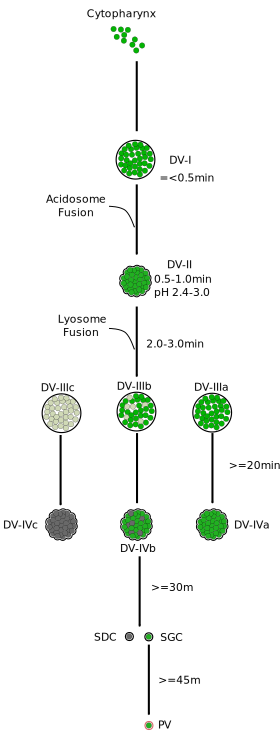
\includegraphics{symbiont_infection.pdf}
\end{figure}
As few as a single algal cell can infect the host \citep{Weis1976} however, the majority of \textit{Chlorella} are digested especially non-competent strains \citep{Kodama2007}. 
Furthermore, it has been established that \textit{Chlorella} strains are fairly host-specific.  
For example, Summerer et al in 2007 \citep{Summerer2007} showed that \textit{Chlorella} isolated from other ciliates were able to establish endosymbioses with \textit{P. bursaria} however, those isolated from cnidarian \textit{Hydra} were not.  
This paper also showed \textit{P. bursaria} favours its symbiotic partner over those isolated from other ciliates when given the choice, this suggests specific adaptations have taken place between host and endosymbiont \citep{Summerer2007}
Free-living \textit{Chlorella} strains do rarely establish endosymbioses with \textit{Paramecium} \citep{Siegel1959}, however they are generally only able to infect fewer \textit{Paramecium} and establish much smaller endosymbiotic populations within the host than the symbiont strains \citep{Siegel1959}

Once established, the symbiosis appears to be mutually beneficial with an observed flux of amino acids and CO$_{2}$ to the endosymbiont and oxygen and photosynthate (principally maltose) to the host as a function of light levels \citep{Karakashian1963}.
The extent of this endosymbiosis is such that \textit{Chlorella} is capable of supporting \textit{Paramecium} in media without its typical bacterial food-stocks and conversely the \textit{Paramecium} is capable of supporting the phototrophic \textit{Chlorella} in the dark for \textasciitilde 2 weeks (or up to 51 endosymbiont cell divisions) suggesting considerable bi-directional nutrient flux \citep{Siegel1960,Karakashian1963}.
It should be noted that for longer periods in the dark or when a bacteria-free culture is used in the dark the host will digest the endosymbionts \citep{Parker1926}
From an ecological perspective, this endosymbiosis can be considered as a means of acquired phototrophy (or mixotrophy), a tactic believed to be advantageous for survival in patchy oligotrophic environments by providing fixed carbon to cover respiration requirements \citep{Putt1990}.
This is largely supported by studies, such as Karkashian's 1963 paper, showing that with a sufficient concentration of bacterial feedstock in the media the growth rate of asymbiotic \textit{Paramecium} ('bleached') and \textit{Paramecium} with \textit{Chlorella} endosymbionts are largely equal.
This threshold is estimated to lie between $10^{6}$ and $10^{7}$ bacteria per ml.  
However, as this is generally a much greater concentration than found in the natural environments of \textit{P. bursaria} the endosymbiosis offers a considerable adaptive advantage to the host \citep{Karakashian1963}
As temporary acquisition of phototrophy is estimated by some research [Raven, 1997] to be less energetically costly than the permanent maintenance of plastids (via endosymbiosis or kleptoplasty) within the host this indicates that this endosymbiosis likely provides other host benefits beyond just the energetics of acquired phototrophy. These include: 
\begin{itemize}
    \item Exploitation of low oxygen environments by the host (as the photosynthesising endosymbiont is capable of providing oxygen to the host \citep{Reisser1980})
\item Photoprotection and protection against 257nm and 282nm UV radiation potentially via endosymbiont pigmentation and localisation to shield host nuclei \citep{Sommaruga2009,Summerer2009,Miwa2009}.  
    This is especially important as the AT-rich \textit{Paramecium} genome is likely prone to UV-damage via the formation of cyclobutane thymine dimers \citep{Sommaruga2009}
\item Protection against predation \citep{Berger1980}. 
    The exact mechanism by which this occurs is unknown, however, it has been observed that mixotrophic ciliates are able to move in rapid `jumping' movements. 
    This is hypothesised as being an energetically costly escape reaction made possible by sugar-rich photosynthate mixotrophic ciliates gain from their algal endosymbionts \citep{Perez1997}. 
    Intriguingly, this protection against predation occurs despite endosymbiont displacement of trichocysts (defensive cellular structures) for attachment to the ciliate cortex \citep{Kodama2011}
    \item Protection against undesired endosymbionts and/or parasites. Algae in \textit{P. bursaria} form an antagonistic relationship with some 
        bacterial endosymbionts but the one specific case %of a un-genetically characterised bacteria is in a russian paper I can't read skobol1982 or something 
        and there is experimental evidence that \textit{P. bursaria} can only be infected by bacteria and yeasts after
\textit{Chlorella} is eliminated \citep{Gortz1982}. This is consistent with bacterial symbionts having been repeatedly identified as providing resistance to parasites in organisms
such as the insects \citep{Martinez2014}
\item Protection against chemical toxins, for example symbiotic \textit{Paramecium} have a much higher survival rate (96\%) to 0.5 mM nickel chloride (NiCl$_{2}$) than asymbiotic \textit{Paramecium} via an undetermined mechanism \citep{Miwa2009}
\item Increased thermotolerance (tested at $42^{o}$C) \citep{Miwa2009}, again, by unknown mechanisms but potentially related to the undefined means of perialgal vacuole attachment to the cell cortex.
\item Protection against excessive oxidative burden (potentially due to endosymbiont dismutases and catalases) \citep{Hortnagl2007a} and hydrogen peroxide (hypothesised by Miwa as being due to the improved energetics of the symbiotic host) \citep{Miwa2009}
\end{itemize}

In return, the endosymbiont also appears to gain several advantages including a generally much increased level of photosynthetic activity \citep{Sommaruga2009}:
\begin{itemize}
    \item CO$_{2}$ from the host \citep{Parker1926}
    \item Nitrogen supply \citep{Johnson2011}.
    \item Amino acids including L-glutamine (likely an important nitrogen source) \citep{Reisser1992} and L-arginine, L-asparagine, L-serine, L-alanine and glycine \citep{Kato2009a}.
    \item Host supplied divalent cations such as K$^{+}$, Mg$^{2+}$, and Ca$^{2+}$. All of which have key roles in photosynthesis \citep{Kato2009a}.
    \item Protection against \textit{Paramecium bursaria – Chlorella} Virus (PBCV) \citep{Yashchenko2012} a large isocahedral dsDNA, 330kbp virus with 133-genes that lyses symbiotic Chlorella when isolated from the host \citep{VanEtten1983}.  This potentially occurs by preventing contact between PBCV and the endosymbiont.
    \item Effective photo-accumulation and increased mobility \citep{Niess1982}.
\end{itemize}
%
This exchange of materials between host and endosymbiont is regulated by an effective biochemical 'bartering' system with numerous feedback cycles. 
For example, the release of endosymbiont photosynthate is dependent on Ca$^{2+}$.  
This ion is provided by the host and also has a role in the up-regulation of photosynthesis (as proxied by oxygen evolution) \citep{Kato2009a}.     
Once photosynthate is released into the PV lumen endosymbiont H$^{+}$-ATPases are activated which allow the generation of the H$^{+}$ gradient necessary for endosymbiont uptake of host-provided amino acids via a set of amino acid-proton symporters (in the same manner as \citep{Camoni2006}) \citep{Kato2009a}.
This proton gradient will potentially lead to further photosynthate release due to observed pH-dependence of this \citep{Kato2009a}. 
As we can see the more photosynthate supplied to the PV lumen the greater the uptake of provided nitrogen sources.  
Intriguingly, from experiments using cycloheximide to selectively interrupt endosymbiont but not host protein synthesis it appears that the maltose transporter that is responsible for export of photosynthate from the PV lumen into the host cytoplasm is endosymbiont derived \citep{Muscatine1967}. 
However, unless photosynthesis is also inhibited (using DCMU) the build up of photosynthate without exportation in the PV triggers the swelling of the vacuole up to 25x its original size.  
This removes the vacuole from the region in which it is protected from lysosome fusion and leads to the digestion of the endosymbiont \citep{Kodama2009a}.
So, here we can see further regulation of the relationship – in which the endosymbiont is degraded if it does not release photosynthate to the host.

On top of this system of secretion, uptake and feedback there have also been several other observed regulatory interactions between host and endosymbiont.  
The most apparent of these are the synchronising of cell division and circadian rhythms between host and endosymbiont with endosymbiotic \textit{Chlorella} sufficient to recover a circadian rhythm in arrhythmic \textit{Paramecium} mutants \citep{Miwa2009}
This regulation of the timing of cell division for both members of the system appears well co-ordinated and takes place in such a way that neither host or endosymbionts outgrow one another \citep{Kadono2004,Takahashi2007}.
The importance of regulation of endosymbiont distribution at host division is evidence in the only natural aposymbiotic \textit{P. bursaria} mutant which
has a impairment in this mechanism and thus can't maintain endosymionts \citep{Tonooka2002}. %good material on algae free in first paragraphs-come back to this paper


\subsection{Separating host and endosymbiont}

naturally aposymbiotic straings of paramecium exist but are rare

artifically reinfecting \citep{Ohkawa2011}
Reduced endsoymbiont numbers:
high radiation doses
excessive food supply
continual darkness with plenty of good - 6 weeks - still some had chlorella so selective picking 6 rimwa  



\section{Conclusion}
In conclusion, understanding the mechanisms by which primary and secondary photosynthetic endosymbioses have occurred is one of the most significant
outstanding problems in understanding the evolution of the eukaryotes. \textit{Paramecium bursaria} and its endosymbiosis with \textit{Chlorella}
offers a useful system to investigate secondary photosynthetic endosymbioses before metabolic co-dependence has become fixed.  
As both organisms seem highly prone to forming endosymbiotic relationships with multiple other organisms as a serial host and serial endosymbiont
respectively it may be possible by identifying the key molecular components of their relationship to understand what factors contribute to such
prolific utilisation of endosymbioses.  Furthermore, while there is considerable supporting literature and many established methodological techniques
for working on these organisms individually and in endosymbiosis there have been relatively scant efforts using the latest -omics techniques 
and reverse genetics such as RNAi.
Considering the historical role both organisms have played independently in our understanding of endosymbiosis\footnote{Margulis was 
    strongly influenced and inspired by research conducted
in organisms closely related to both \textit{Paramecium bursaria} and 
\textit{Micractinium reisseri}. Specifically, the discovery of Tracey Sonneborn
of non-mendelian cytoplasmic inheritance in \textit{Paramecium bursaria} \citep{Sonneborn1950}
and the multiple lines of evidence of the presence of DNA within the chloroplasts
gleaned from several species of green algae related to \textit{Micractinium reisseri}
(\textit{Spriogyra} \citep{Stocking1959}, \textit{Chalymdomonas moewussii}, and 
\textit{Chlorella ellipsoidea} \cite{Ris1962}).} it is perhaps apt that further insight may be gleaned by applying the latest modern 
techniques to interrogate their relationship.

%% Mieosis turned off  ehhh???
z
